%%%%%%%%%%%%%%%%%%%%%%%%%%%%%%%%%%%%%%%%%
% Journal Article
% LaTeX Template
% Version 1.4 (15/5/16)
%
% This template has been downloaded from:
% http://www.LaTeXTemplates.com
%
% Original author:
% Frits Wenneker (http://www.howtotex.com) with extensive modifications by
% Vel (vel@LaTeXTemplates.com)
%
% License:
% CC BY-NC-SA 3.0 (http://creativecommons.org/licenses/by-nc-sa/3.0/)
%
%%%%%%%%%%%%%%%%%%%%%%%%%%%%%%%%%%%%%%%%%

%----------------------------------------------------------------------------------------
%	PACKAGES AND OTHER DOCUMENT CONFIGURATIONS
%----------------------------------------------------------------------------------------

\documentclass[twoside,twocolumn]{article}

\usepackage{blindtext} % Package to generate dummy text throughout this template 

\usepackage[sc]{mathpazo} % Use the Palatino font
\usepackage[T1]{fontenc} % Use 8-bit encoding that has 256 glyphs
\linespread{1.05} % Line spacing - Palatino needs more space between lines
\usepackage{microtype} % Slightly tweak font spacing for aesthetics

\usepackage[english]{babel} % Language hyphenation and typographical rules

\usepackage[hmarginratio=1:1,top=32mm,columnsep=20pt]{geometry} % Document margins
\usepackage[hang, small,labelfont=bf,up,textfont=it,up]{caption} % Custom captions under/above floats in tables or figures
\usepackage{booktabs} % Horizontal rules in tables

\usepackage{lettrine} % The lettrine is the first enlarged letter at the beginning of the text

\usepackage{enumitem} % Customized lists
\setlist[itemize]{noitemsep} % Make itemize lists more compact

\usepackage{abstract} % Allows abstract customization
\renewcommand{\abstractnamefont}{\normalfont\bfseries} % Set the "Abstract" text to bold
\renewcommand{\abstracttextfont}{\normalfont\small\itshape} % Set the abstract itself to small italic text

\usepackage{titlesec} % Allows customization of titles
\renewcommand\thesection{\Roman{section}} % Roman numerals for the sections
\renewcommand\thesubsection{\roman{subsection}} % roman numerals for subsections
\titleformat{\section}[block]{\large\scshape\centering}{\thesection.}{1em}{} % Change the look of the section titles
\titleformat{\subsection}[block]{\large}{\thesubsection.}{1em}{} % Change the look of the section titles

\usepackage{fancyhdr} % Headers and footers
\pagestyle{fancy} % All pages have headers and footers
\fancyhead{} % Blank out the default header
\fancyfoot{} % Blank out the default footer
\fancyhead[C]{Harvey Hughes $\bullet$ November 2019 $\bullet$ Emmanuel College} % Custom header text
\fancyfoot[RO,LE]{\thepage} % Custom footer text

\usepackage{titling} % Customizing the title section

\usepackage{hyperref} % For hyperlinks in the PDF

\usepackage{graphicx}
\graphicspath{ {images/} }

\newenvironment{reusefigure}[2][htbp]
  {\addtocounter{figure}{-1}%
   \renewcommand{\theHfigure}{dupe-fig}% If you're using hyperref
   \renewcommand{\thefigure}{\ref{#2}}% Figure counter is \ref
   \renewcommand{\addcontentsline}[3]{}% Avoid placing figure in LoF
   \begin{figure}[#1]}
  {\end{figure}}
\usepackage{wrapfig}
\usepackage{amsmath}
\usepackage{xcolor}
\usepackage{listings}
\usepackage{subcaption}
\usepackage{pdfpages}
\usepackage{array,multirow,graphicx}
\lstset{
  basicstyle=\ttfamily,
  columns=fullflexible,
  frame=single,
  breaklines=true,
  postbreak=\mbox{\textcolor{red}{$\hookrightarrow$}\space},
}

%----------------------------------------------------------------------------------------
%	TITLE SECTION
%----------------------------------------------------------------------------------------

\setlength{\droptitle}{-4\baselineskip} % Move the title up

\pretitle{\begin{center}\Huge\bfseries} % Article title formatting
\posttitle{\end{center}} % Article title closing formatting
\title{4F13 - Coursework One - Gaussian Processes } % Article title
\author{%
\\
\textsc{Candidate Number: 5584F} \\
\normalsize Word count: 998 \\
}
\date{\today} % Leave empty to omit a date
\renewcommand{\maketitlehookd}{%
}

%----------------------------------------------------------------------------------------

\begin{document}
\onecolumn
\includepdf[pages={1}]{coversheet.pdf}
\twocolumn
% Print the title
\maketitle

%----------------------------------------------------------------------------------------
%	ARTICLE CONTENTS
%----------------------------------------------------------------------------------------


\section{a}
\begin{figure}[h]
  \centering
    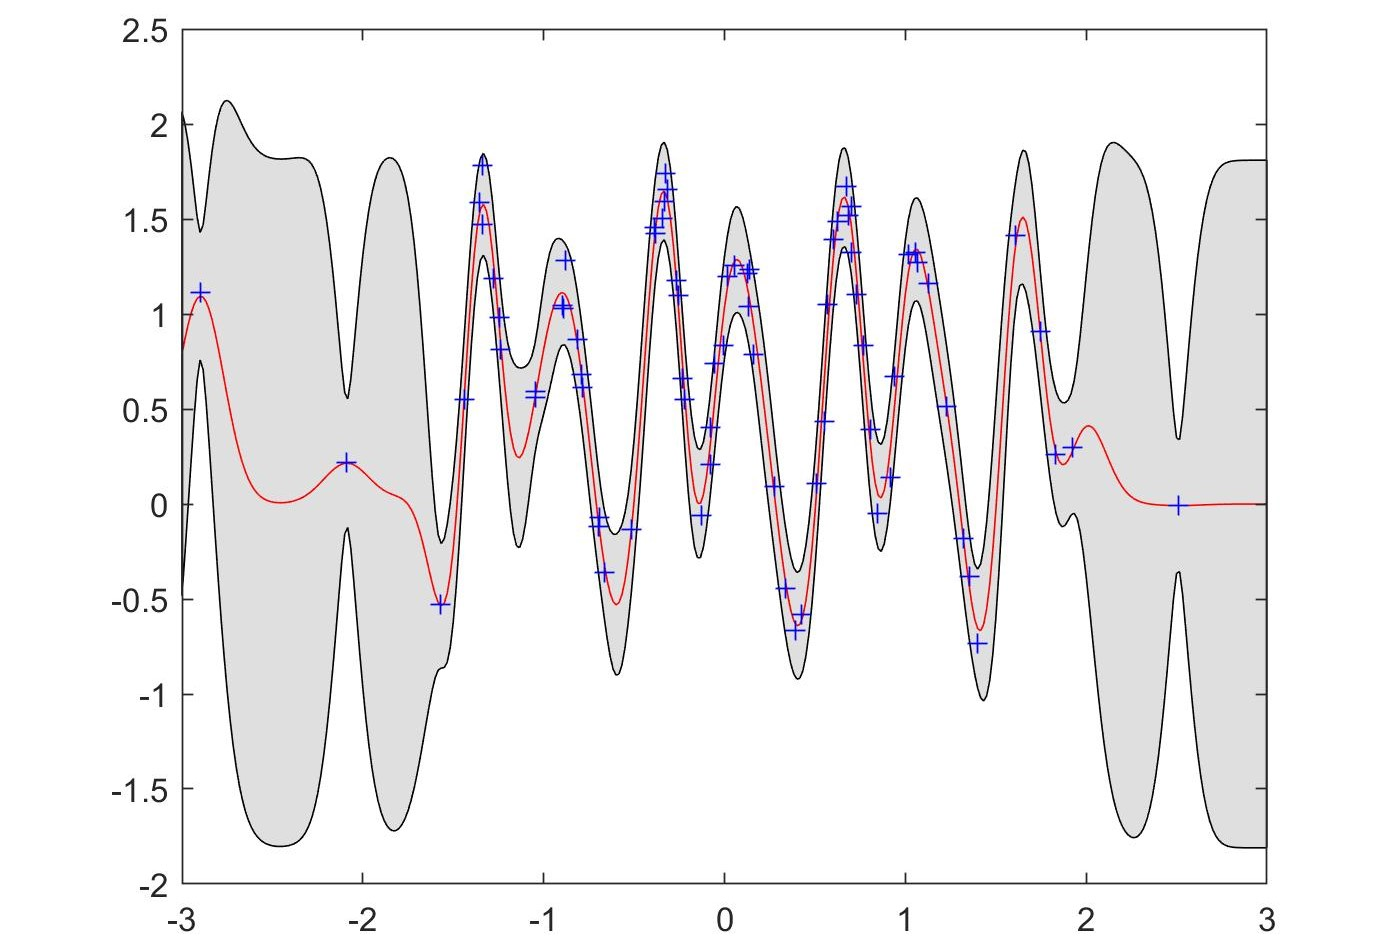
\includegraphics[width=\linewidth]{c_1_1}
  \caption{GP with squared exponential covariance trained on data a with log hyper parameters initialised at [-1, 0, 0]}
  \label{fig:c_1}
\end{figure}
Figure \ref{fig:c_1} shows the result of training a GP with squared exponential covariance function with log hyper parameters initialised at [-1, 0, 0]. After minimisation of negative log marginal likelihood ( -log[p(y|x,$\mathcal{M}$)] ) the hyper parameters ($\boldsymbol{\theta}$) were [0.1282 ,0.897, 0.1178] which corresponds to characteristic length scale, signal $\sigma$ and noise $\sigma$ respectively. The optimised log[p(y|x,$\mathcal{M}$)] was -11.9. The hyper parameters are observed in figure \ref{fig:c_1} as the length scale representing feature size in the x direction, signal $\sigma$ the feature amplitude, and noise $\sigma$ the data variation about the mean. The 95\% error bars are very thin where data is observed corresponding to a high likelihood of the function existing here, at the extremes data is more sparse so the uncertainty in function shape is greater.
\newline
All essential code listing can be seen in the appendix.
%------------------------------------------------
\section{b}
Additional local minima in negative log marginal likelihood can be located from different initialisations. Figure \ref{fig:hyp} shows four of these local minima, and their respective log[p(y|x,$\mathcal{M}$). Figure \ref{sub:hyp1} shows a fit with length scale 8 which is more then the observed range. This causes large uncertainties and is only able to only capture the downward trend. Figure \ref{sub:hyp2} extends this length scale even further to the point where the model believes a constant but very noisy function is correct. Figure \ref{sub:hyp3} shows a model of very small length scale, the mean passes through the data very well but its very noisy between data points. Figure \ref{sub:hyp4} shows a similar model to the initial one, but with smaller signal $\sigma$ and therefore smaller confidence intervals.
\newline
By looking at the log marginal likelihood you can assess how good a fit the model is, the best two being figures \ref{fig:c_1} and \ref{sub:hyp4}. Both these appear to fit the data equally well without overfitting, but due to the still significantly higher log[p(y|x,$\mathcal{M}$)] of figure \ref{fig:c_1} this model is likely to be the best fit.
\begin{figure*}[h]
\centering
    \begin{subfigure}[t]{0.49\linewidth}
        \centering
        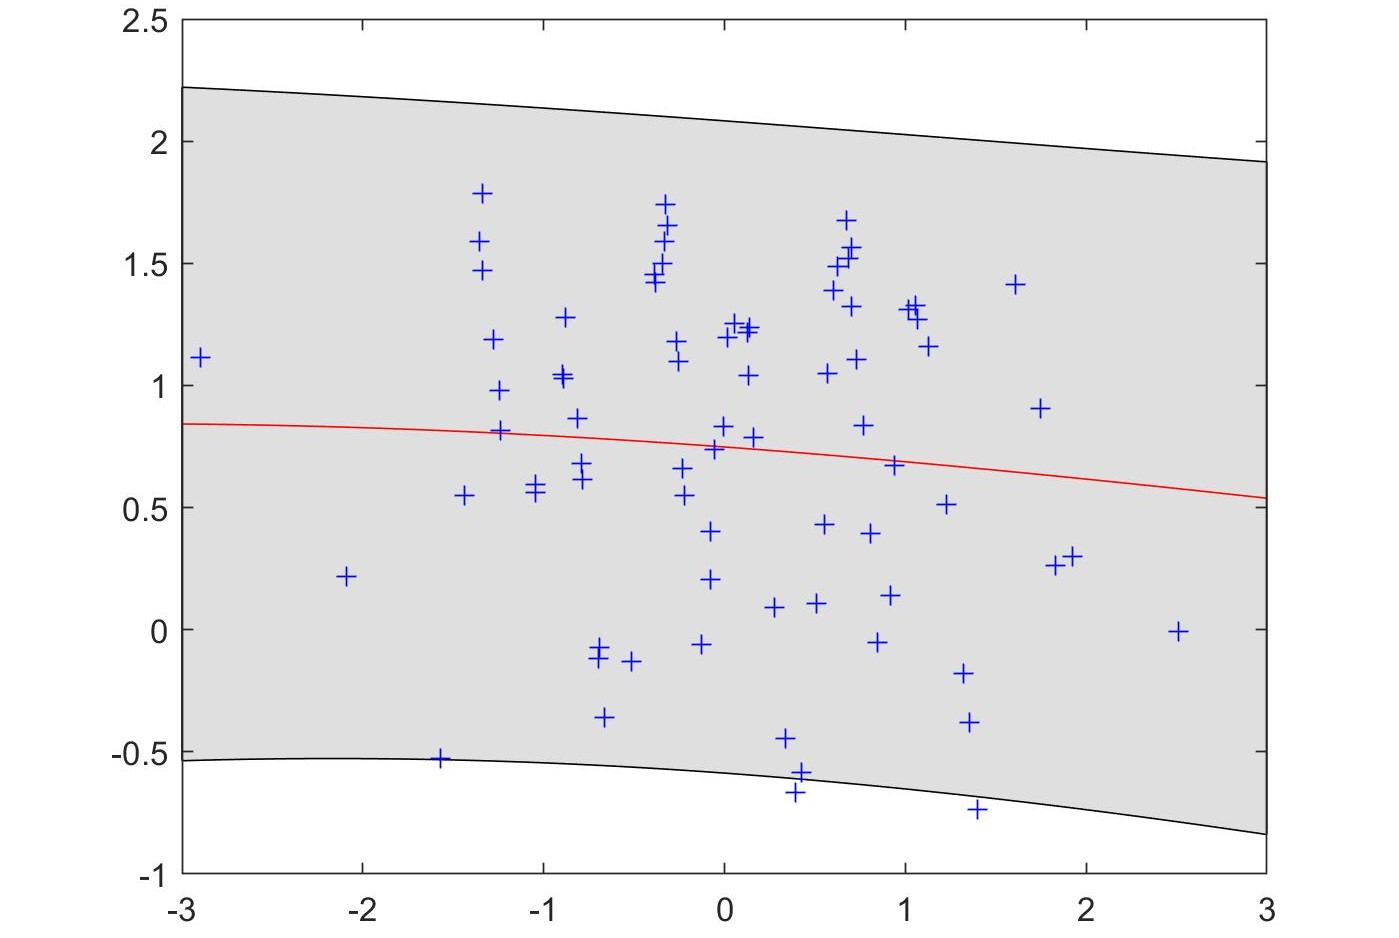
\includegraphics[width=\textwidth]{c_1_2_1_graph}
        \caption{\textbf{$\theta$} = [8.042, 0.696, 0.663], log[p(y|x,$\mathcal{M}$)] = -78.22}
        \label{sub:hyp1}
    \end{subfigure}%
    \begin{subfigure}[t]{0.49\linewidth}
        \centering
        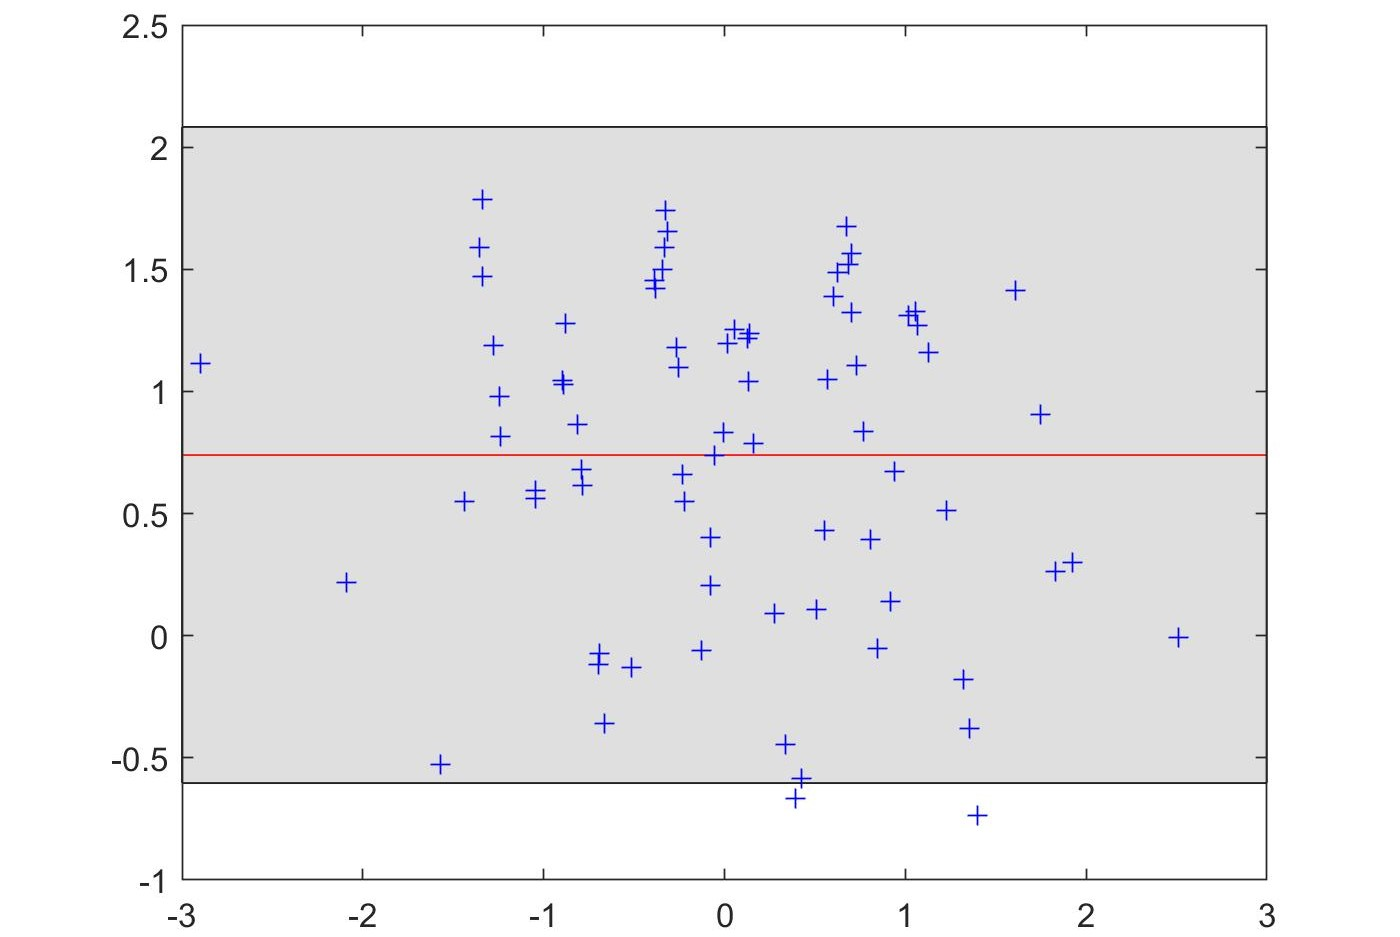
\includegraphics[width=\textwidth]{c_1_2_3_graph}
        \caption{\textbf{$\theta$} = [3.3e10, 0.744, 0.667], log[p(y|x,$\mathcal{M}$)] = -78.34}
        \label{sub:hyp2}
    \end{subfigure}%
    \newline
    \begin{subfigure}[t]{0.49\linewidth}
        \centering
        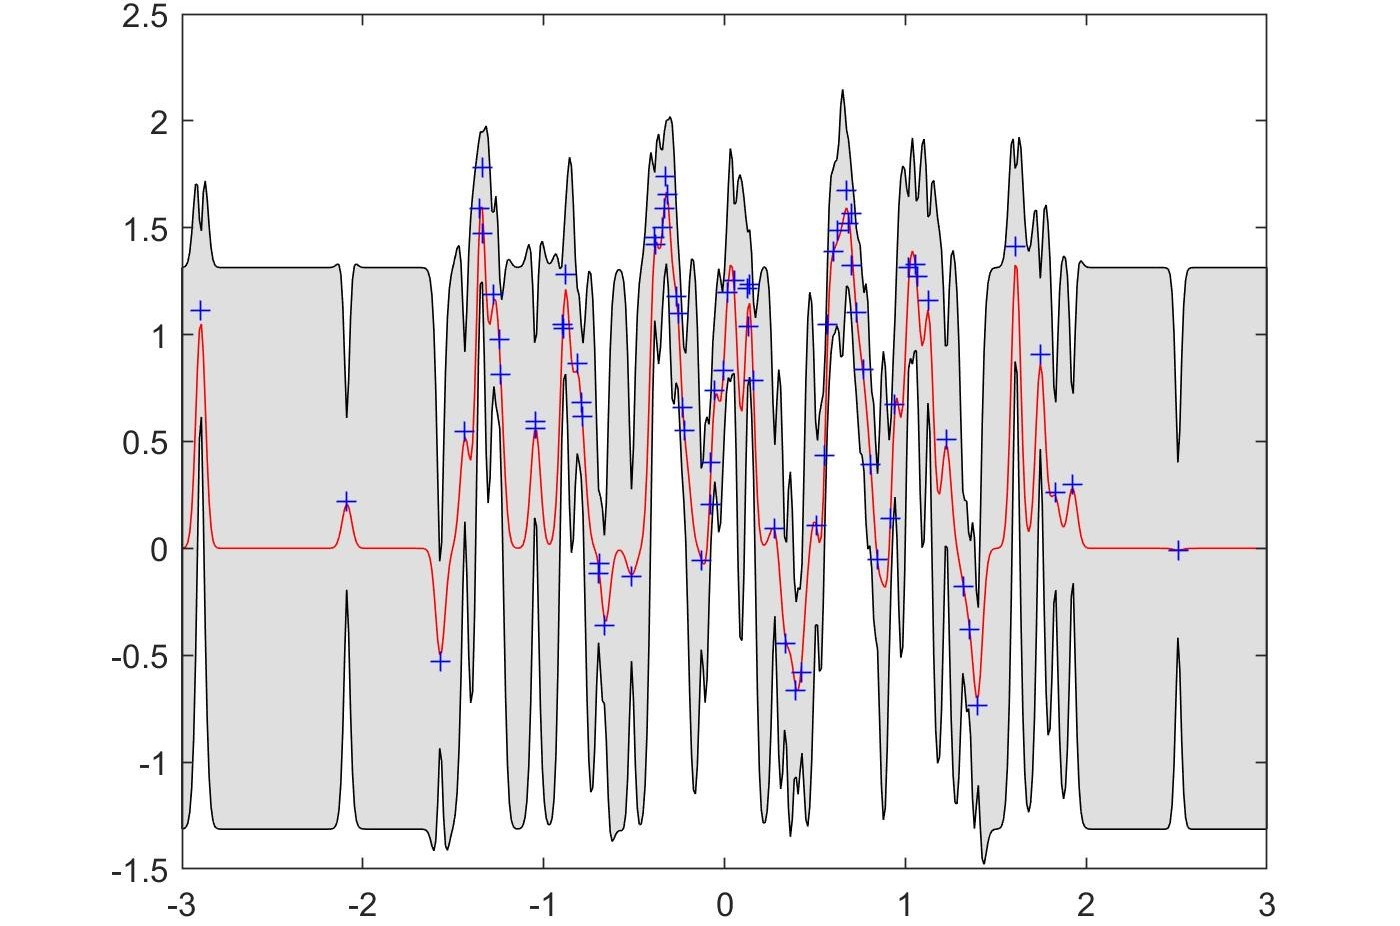
\includegraphics[width=\textwidth]{c_1_2_4_graph}
        \caption{\textbf{$\theta$} = [0.0263, 0.641, 0.142], log[p(y|x,$\mathcal{M}$)] = -57.56} 
        \label{sub:hyp3}
    \end{subfigure}
    \begin{subfigure}[t]{0.49\linewidth}
        \centering
        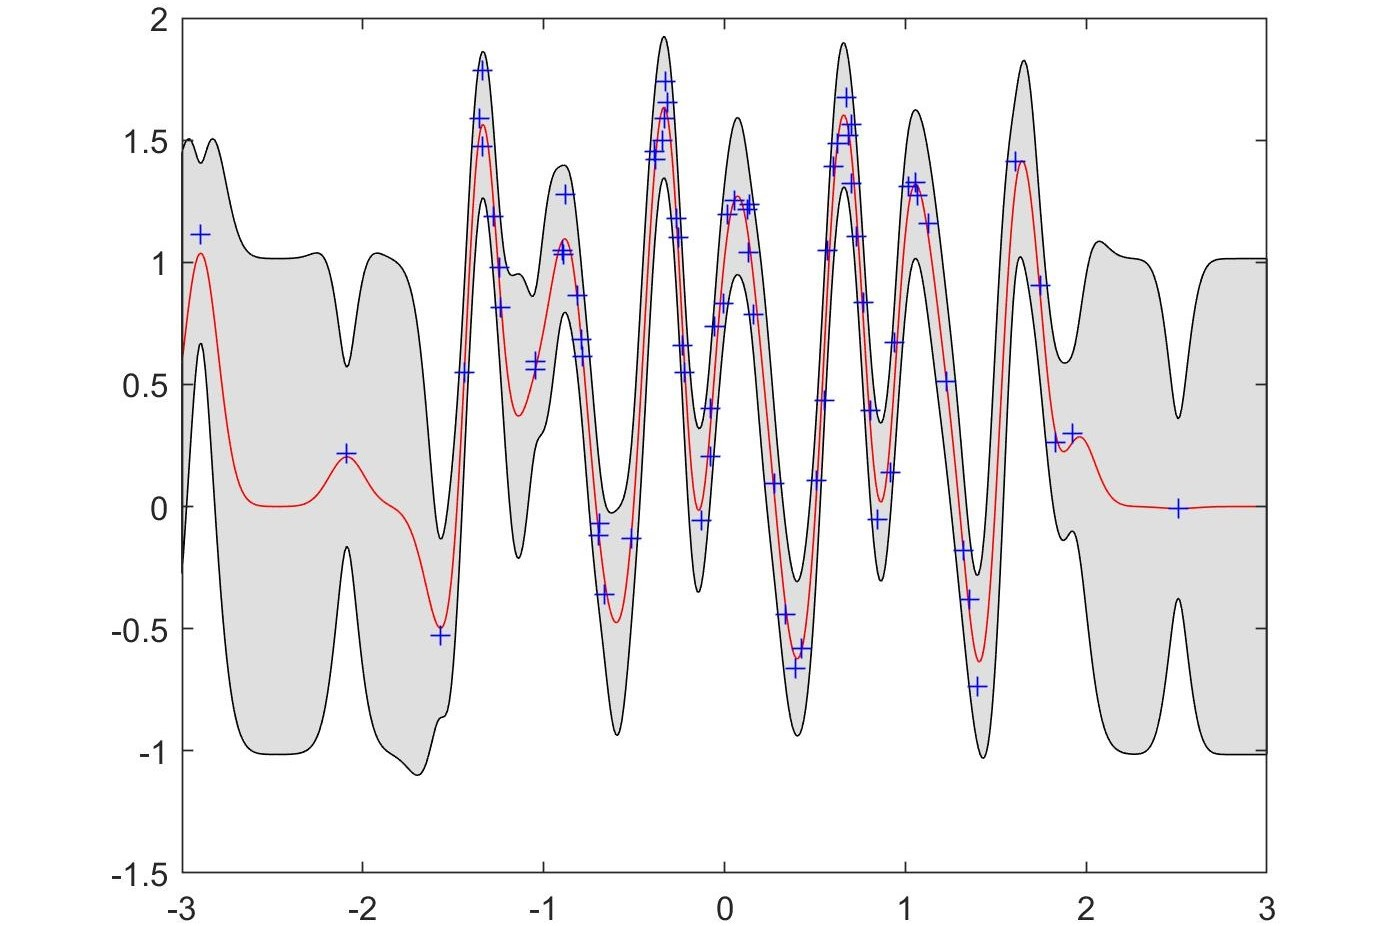
\includegraphics[width=\textwidth]{c_1_2_5_graph}
        \caption{\textbf{$\theta$} = [0.097, 0.49, 0.132], log[p(y|x,$\mathcal{M}$)] = -23.46}
        \label{sub:hyp4}
    \end{subfigure}
    \caption{The effect of different hyper parameters}
    \label{fig:hyp}
\end{figure*}

\begin{figure}[h]
  \centering
    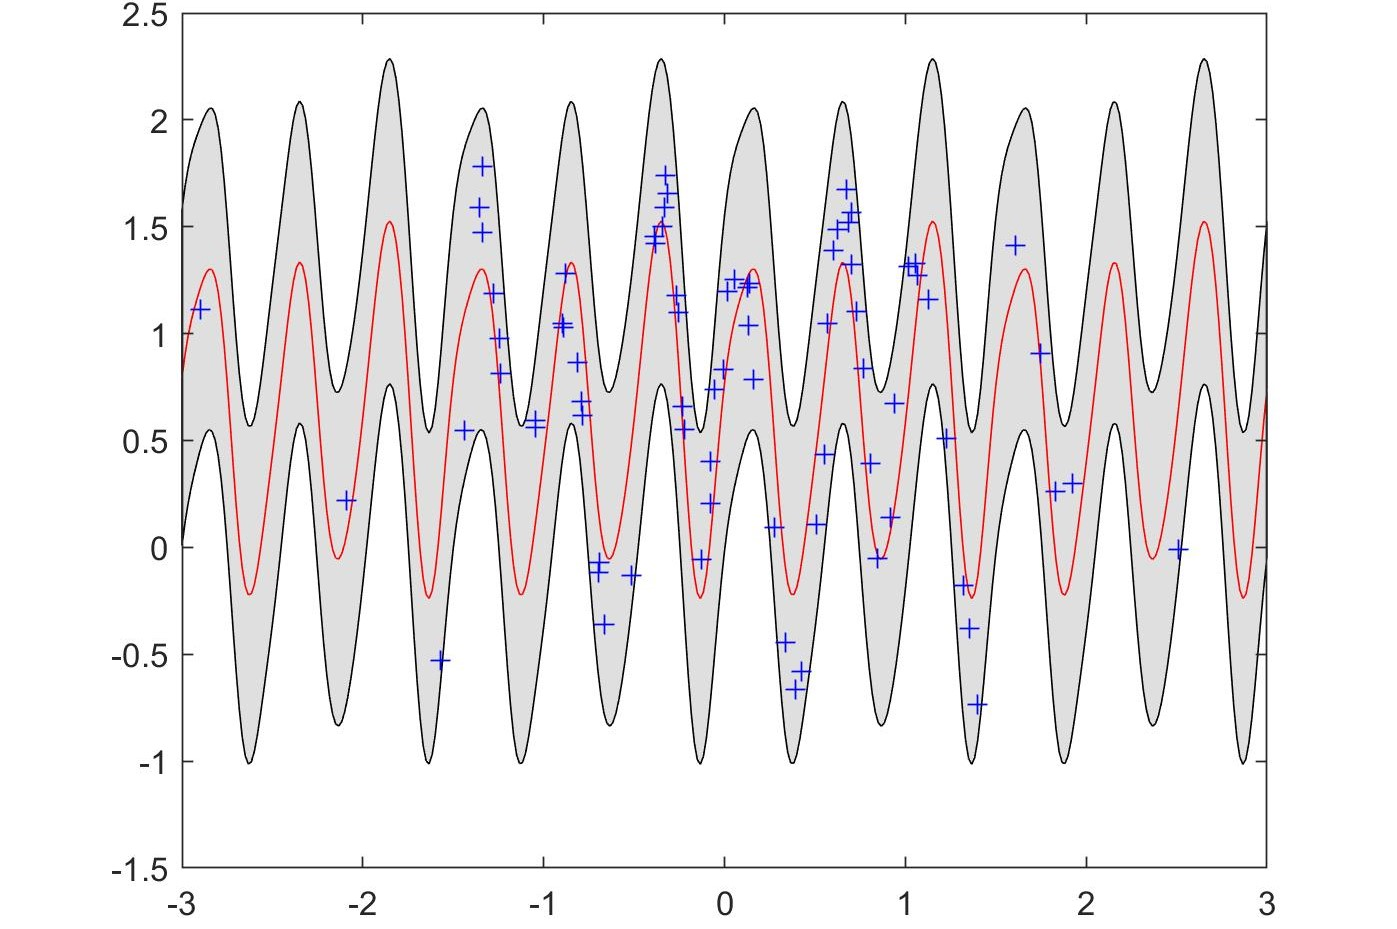
\includegraphics[width=\linewidth]{c_1_3_1}
  \caption{Periodic covariance with \textbf{$\theta$} = [0.49, 1.5, 1.17, 0.356], log[p(y|x,$\mathcal{M}$)] = -48.1}
  \label{fig:per1}
\end{figure}

\begin{figure}[h]
  \centering
    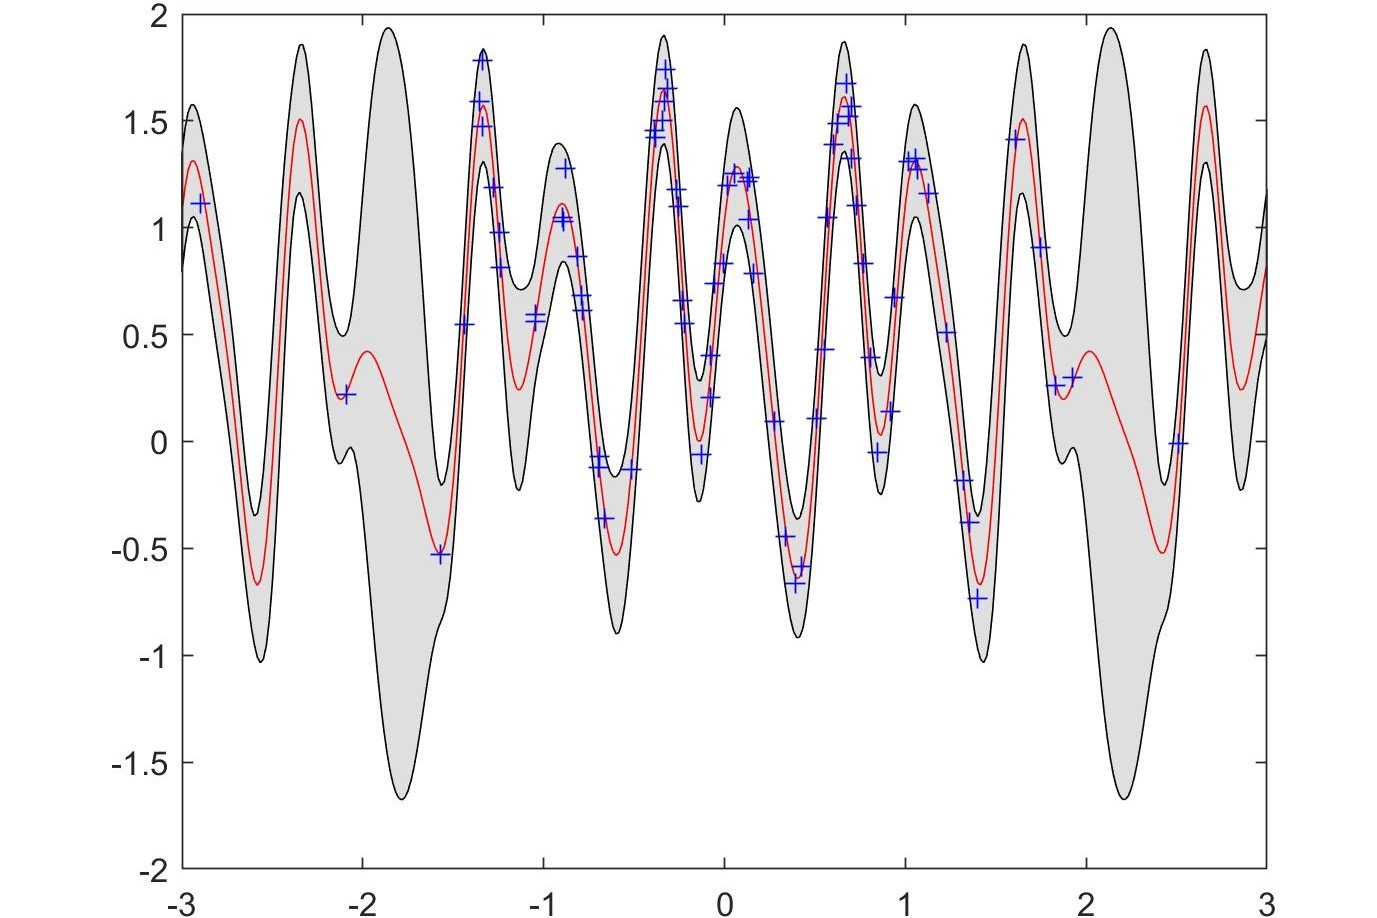
\includegraphics[width=\linewidth]{c_1_3_2}
  \caption{Periodic covariance with \textbf{$\theta$} = [0.205, 4.0, 0.93, 0.116], log[p(y|x,$\mathcal{M}$)] = -6.7}
  \label{fig:per2}
\end{figure}

\begin{figure*}[h]
\centering
    \begin{subfigure}[t]{0.49\linewidth}
        \centering
        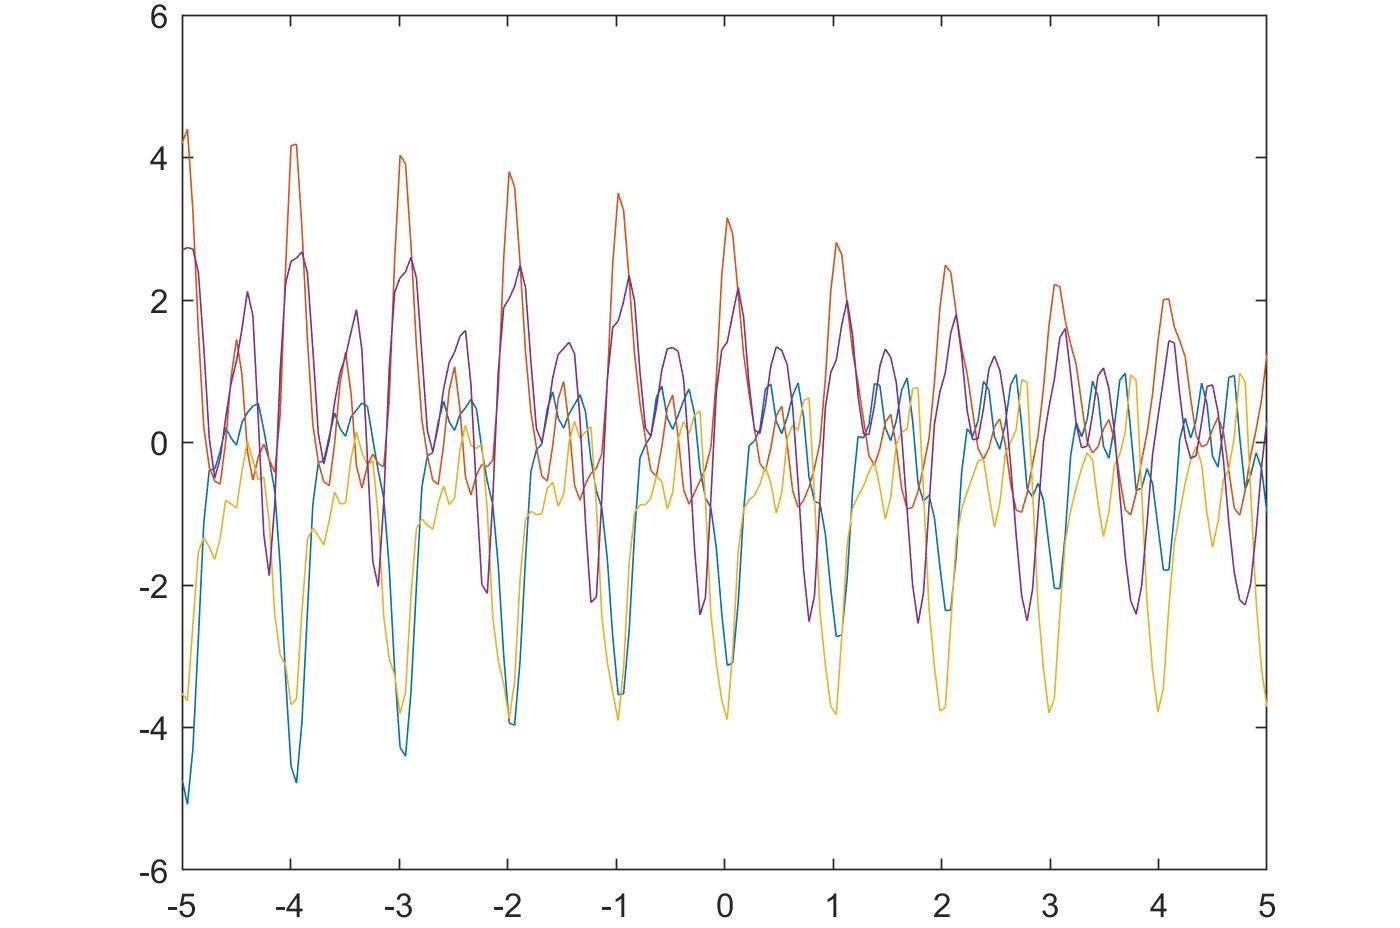
\includegraphics[width=\textwidth]{c_1_4_1}
        \caption{4 Functions}
        \label{sub:r1}
    \end{subfigure}%
    \begin{subfigure}[t]{0.49\linewidth}
        \centering
        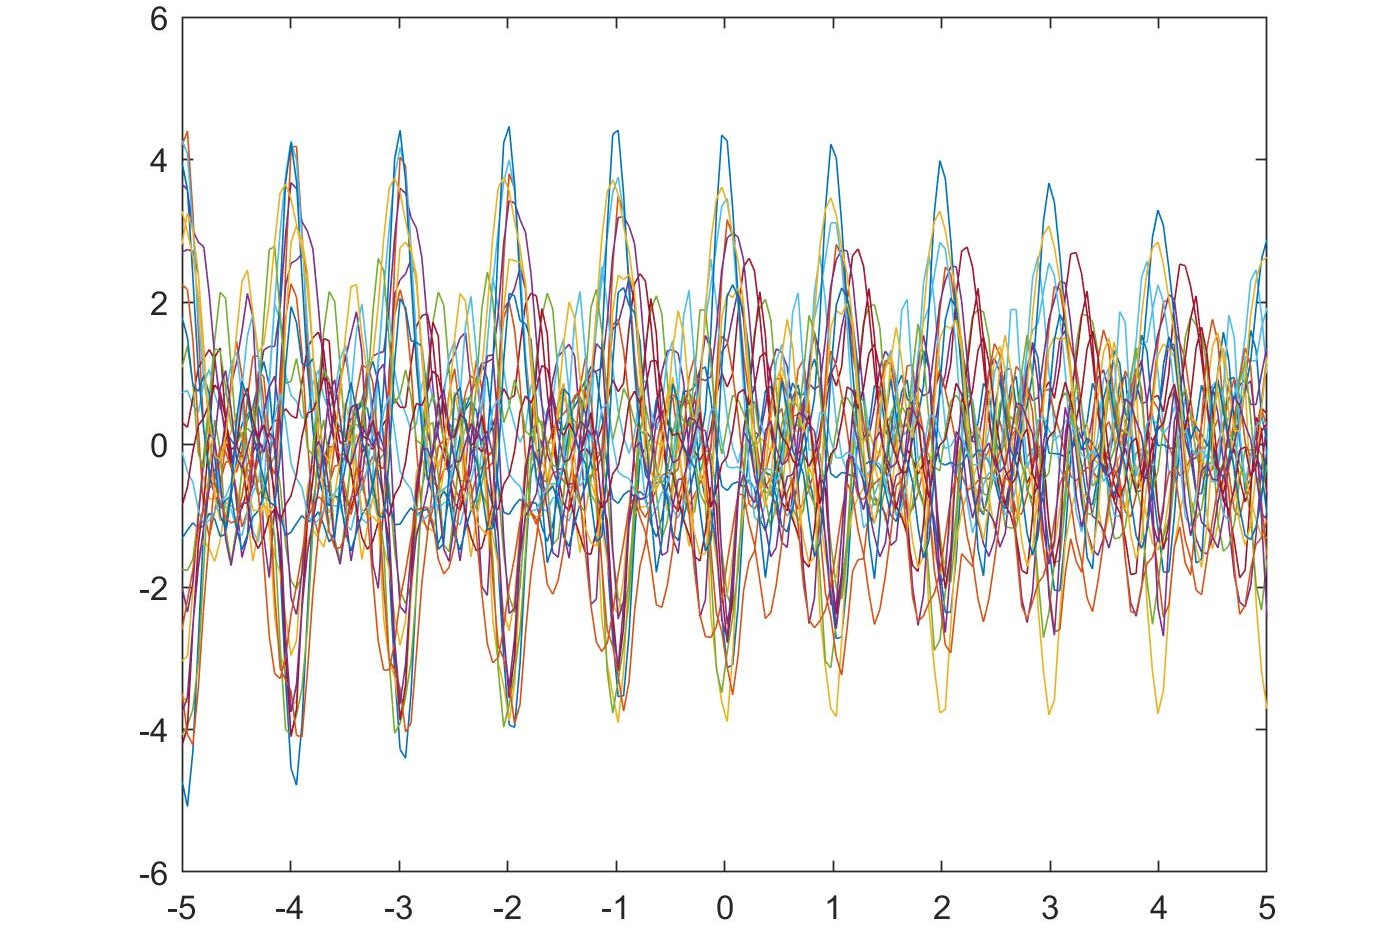
\includegraphics[width=\textwidth]{c_1_4_2}
        \caption{25 Functions}
        \label{sub:r2}
    \end{subfigure}%
    \newline
    \begin{subfigure}[t]{0.49\linewidth}
        \centering
        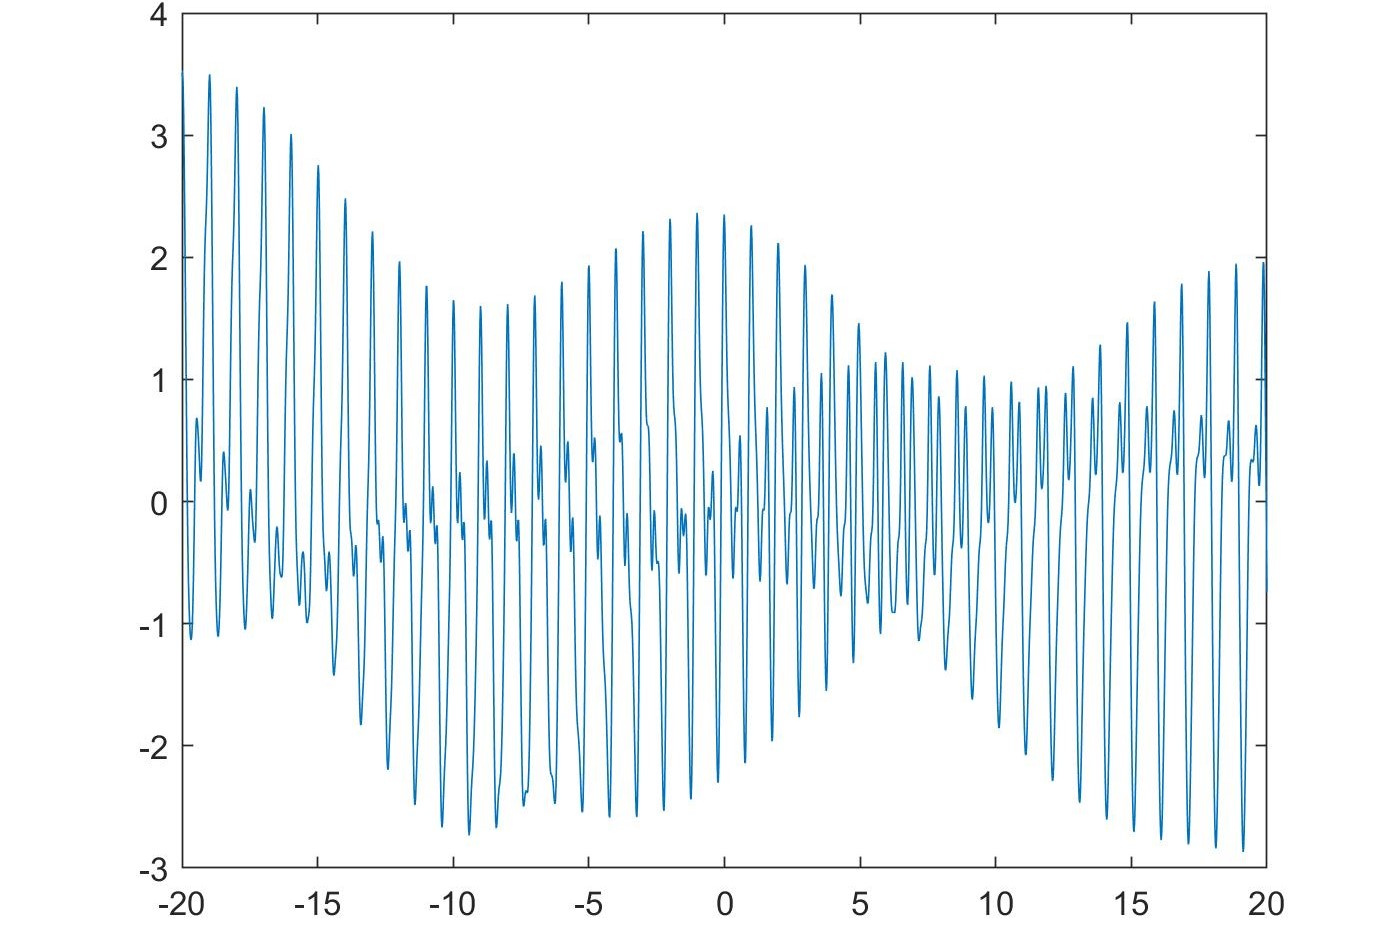
\includegraphics[width=\textwidth]{c_1_4_3}
        \caption{Wider range}
        \label{sub:r3}
    \end{subfigure}%
    \caption{Various random functions}
    \label{fig:ran}
\end{figure*}
%------------------------------------------------
\section{c}
The same data was modelled using a periodic covariance function, this requires an additional hyper parameter ($\theta$[2]) for the period. Figures \ref{fig:per1} and \ref{fig:per2} show these models. By using a periodic covariance function the model gains prior information. This means that in regions of low data around x=$\pm$2.5 the model still shows small error bars compared to using a squared exponential covariance as before. Increasing signal $\sigma$ from figure \ref{fig:per1} to \ref{fig:per2} reduces the error bars, models the peaks better and increases log[p(y|x,$\mathcal{M}$)] to above that of the squared exponential models. This higher likelihood and small predictive error bars at extremes makes me believe the data was generated periodically. However, shown in figure \ref{sub:hyp1} there is a general negative trend in the data which isn't periodic, meaning the generation could be a combination of periodic and linear terms.



%------------------------------------------------
\section{d}
Random functions can be generated using desired covariance functions, figure \ref{fig:ran} shows some sample functions using the covariance function in equation \ref{eq:cov}, and hyper parameters [$L_p,p,S_{\sigma p},L_s,S_{\sigma s}$] = [0.606, 1, 1, 7.39, 1]. When generating a small diagonal matrix must be added to the covariance matrix, this is to ensure the matrix is positive semi-definite. Rounding errors can cause small negative eigenvalues which this addition corrects. Positive semi-definite covariance matrices ensure the probability distribution assigns positive mass to all values and therefore is valid.

\begin{equation}
k(x,z)= S_{\sigma p}^2S_{\sigma s}^2 exp(\frac{-2Sin^2\frac{\pi(x-z)}{p}}{L_p^2} -\frac{(x-z)^2}{2L_s^2} )
\label{eq:cov}
\end{equation}

The parameters can be observed in the functions in figure \ref{fig:ran}. The period of 1 is the distance between the large peaks. The characteristic length scales can be seen in figure \ref{sub:r3}, 7.39 is the squared exponential scale and determines envelope frequency, and 0.606 is the small variation between the main periods. The signal $\sigma$ of both parts is 1 and is the size of these variations.

\begin{figure*}[h]
\centering
    \begin{subfigure}[t]{0.49\linewidth}
        \centering
        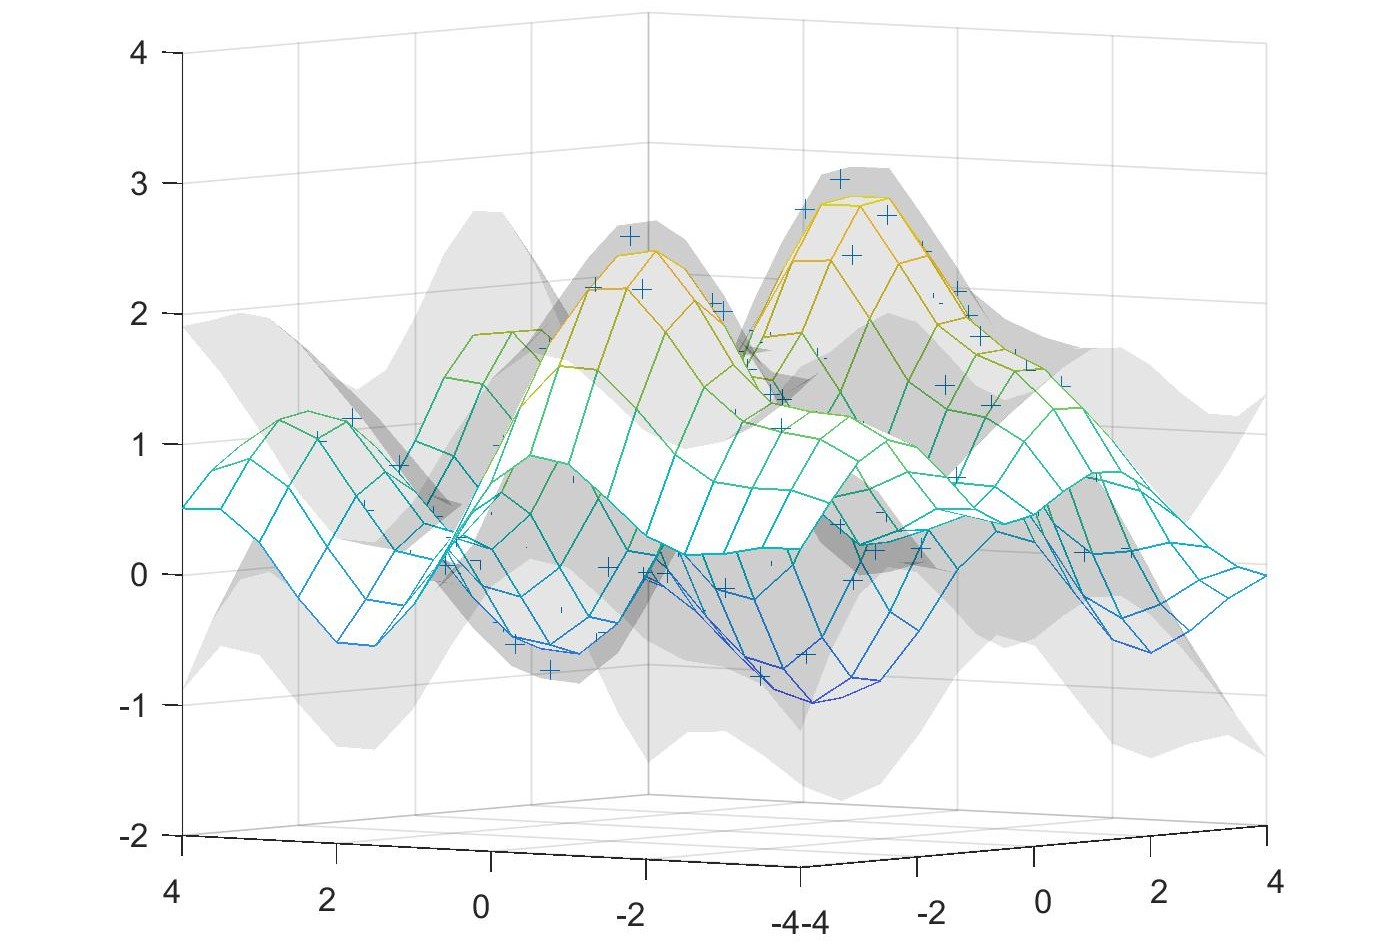
\includegraphics[width=\textwidth]{c_1_5_1}
        \caption{Model 1 3D plot}
        \label{sub:2d1}
    \end{subfigure}%
    \begin{subfigure}[t]{0.49\linewidth}
        \centering
        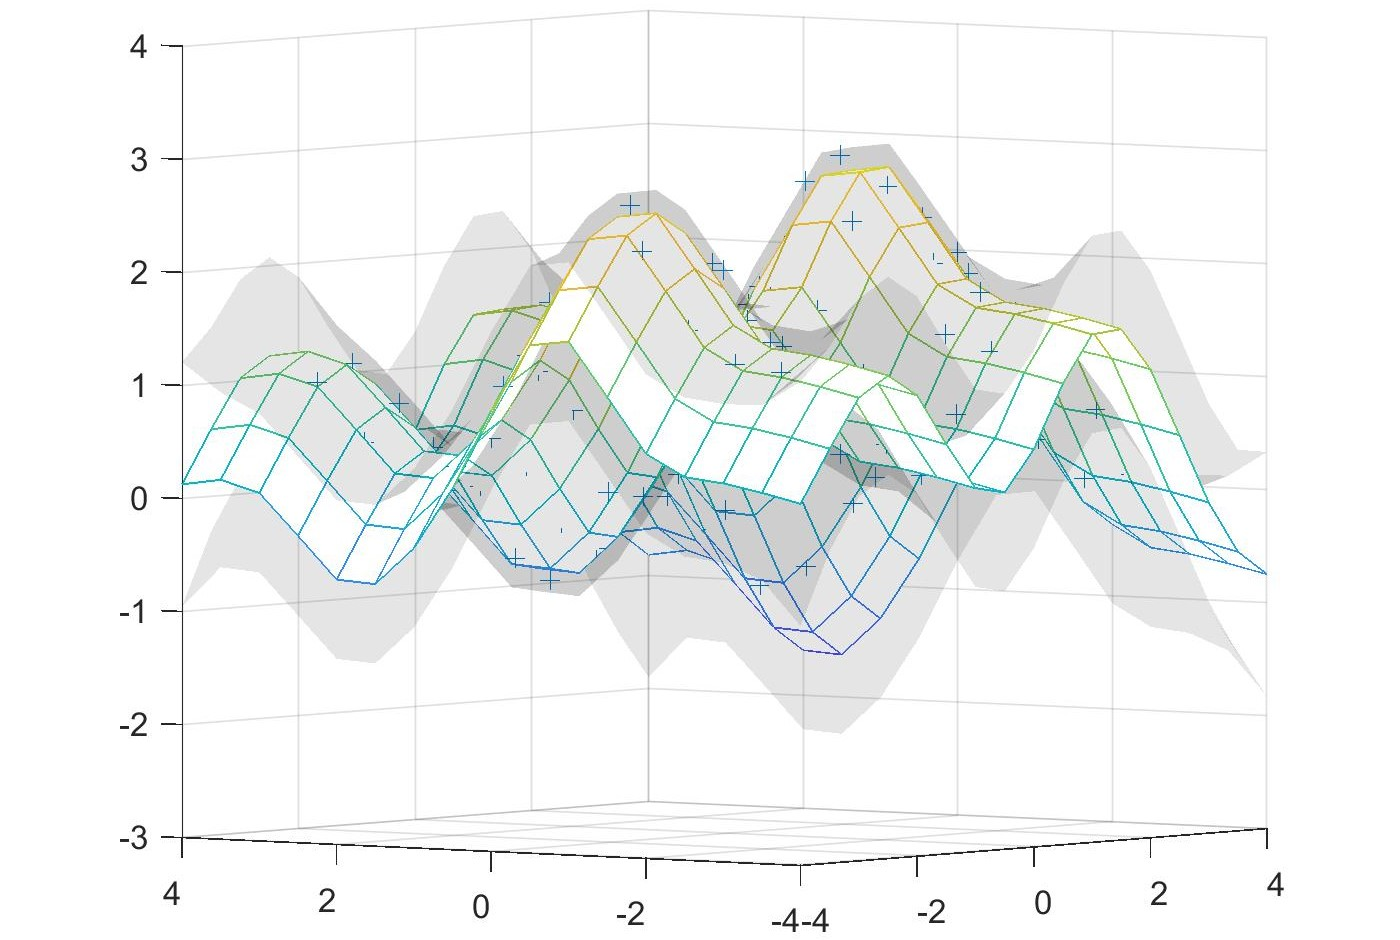
\includegraphics[width=\textwidth]{c_1_5_2}
        \caption{Model 2 3D plot}
        \label{sub:2d2}
    \end{subfigure}%
    \newline
    \begin{subfigure}[t]{0.49\linewidth}
        \centering
        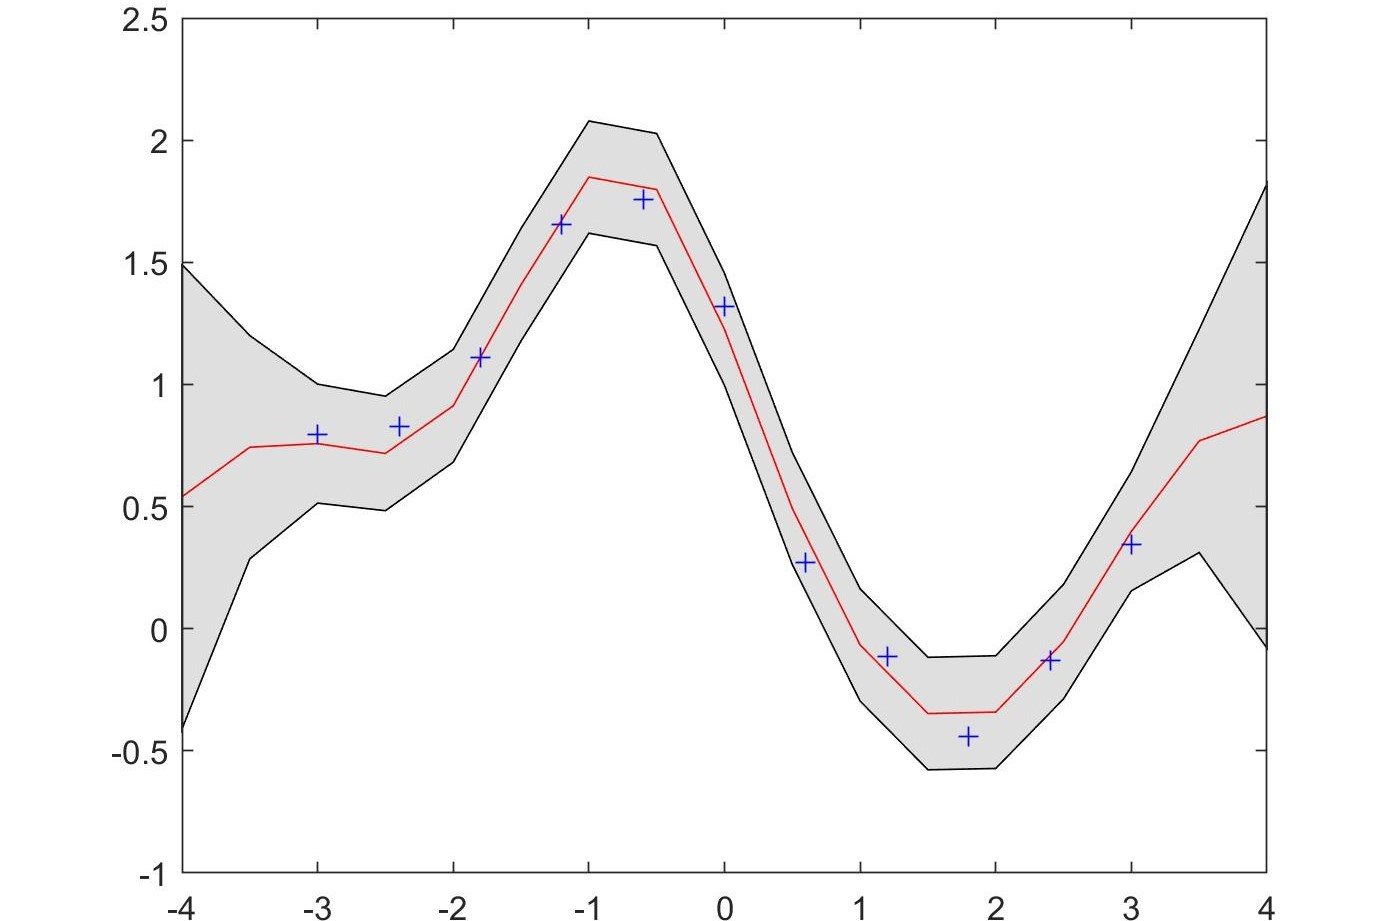
\includegraphics[width=\textwidth]{c_1_5_3}
        \caption{Model 1 slice through x(1) = 0} 
        \label{sub:2d3}
    \end{subfigure}
    \begin{subfigure}[t]{0.49\linewidth}
        \centering
        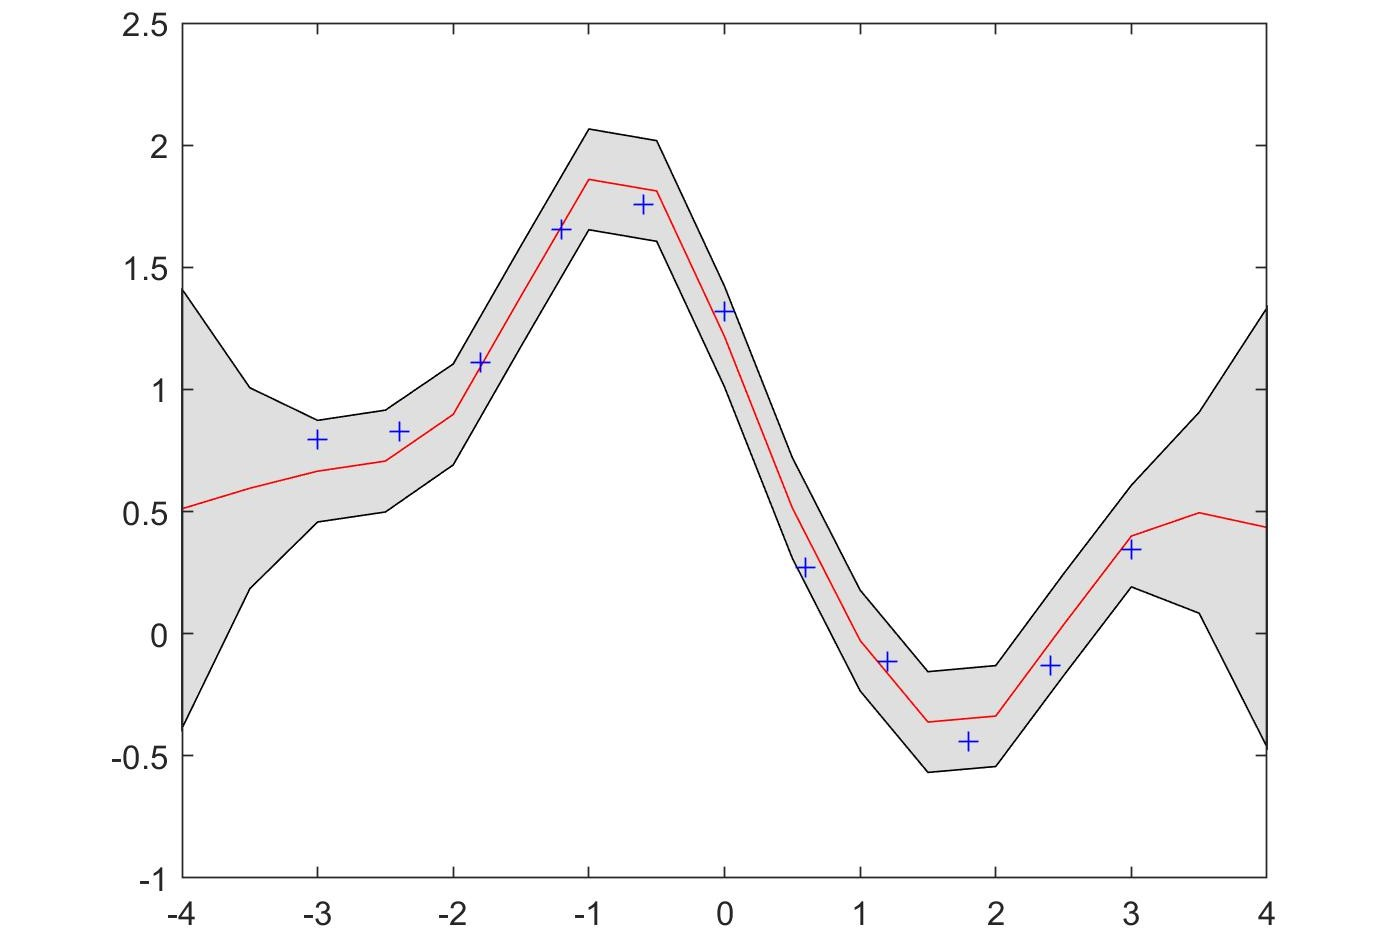
\includegraphics[width=\textwidth]{c_1_5_4}
        \caption{Model 2 slice through x(1) = 0}
        \label{sub:2d4}
    \end{subfigure}
    \caption{Visualisations of two models on the 2D data}
    \label{fig:2d}
\end{figure*}
%------------------------------------------------------
\section{e}
Two dimensional data was loaded and modelled using two models of varying complexity. The covariance functions are shown in equations \ref{eq:cov2} and \ref{eq:cov3}. The resulting log[p(y|\textbf{x},$\mathcal{M}$)], and sum of uncertainty is listed in table \ref{table:2d}. Visually both models  fit the data well, however the additional term is shown to increase the likelihood significantly meaning the extra complexity is worthwhile. The additional complexity also doesn't run into the problems of over fitting as marginally likelihood accounts for this. Additional models with more terms in the covariance function were tested, but these showed no further improvements. 

\begin{equation}
k_1(x,z)= S_{\sigma s}^2 exp(-\frac{(x-z)^T
\begin{bmatrix}
L_1^2 0 \\
0 L_2^2
\end{bmatrix}^{-1}
(x-z)}{2})
\label{eq:cov2}
\end{equation}

\begin{equation}
k_2(x,z)= k_1(x,z) + k_1(x,z)
\label{eq:cov3}
\end{equation}

\begin{table}[h]
\centering
\begin{tabular}{ c | c | c }
Model&log[p(y|\textbf{x},$\mathcal{M}$)]&$\Sigma_1^D \sigma_y^2$\\ 

\midrule
One&19.219&20.18\\
Two&66.408&14.9\\
Three&66.404&14.89 \\
Four&66.403&14.9\\
Five&66.40&14.87\\
Six&66.40&14.94\\


\end{tabular}
\caption{Model Performance}
\label{table:2d}
\end{table}
\section{Appendix - Code listings}
\subsection{a,b,c}
\begin{lstlisting}[language=matlab]
meanfunc = [];                     
covfunc = @covSEiso;              
likfunc = @likGauss;              
hyp = struct('mean', [], 'cov', [-1 0], 'lik', 0);
hyp2 = minimize(hyp, @gp, -100, @infGaussLik, meanfunc, covfunc, likfunc, x, y);
  [mu s2] = gp(hyp2, @infGaussLik, meanfunc, covfunc, likfunc, x, y, xs);
\end{lstlisting}

\subsection{d}
\begin{lstlisting}[language=matlab]
 x= linspace(-5,5,200)';
 K = feval(covfunc{:}, hyp.cov, x);
  for i = 1:25
    x2 = gpml_randn(2, 200, 1);
    y = chol(K+1e-6*eye(200))'*x2 ;
    plot(x, y)
    hold on
  end
\end{lstlisting}
\subsection{e}
\begin{lstlisting}[language=matlab]
%3D plotting
figure(2);
[mu2 s2] = gp(hyp2min, @infGaussLik, meanfunc, covfunc2, likfunc, x, y, xs);
mesh(reshape(xs(:,1),17,17),reshape(xs(:,2),17,17),reshape(mu2,17,17));
hold on;
scatter3(x(:,1),x(:,2), y, '+');
hold on;
surf(reshape(xs(:,1),17,17),reshape(xs(:,2),17,17),reshape(mu2+2*sqrt(s2),17,17),'FaceAlpha','0.1','EdgeColor' , 'none','FaceColor','k');
hold on;
surf(reshape(xs(:,1),17,17),reshape(xs(:,2),17,17),reshape(mu2-2*sqrt(s2),17,17),'FaceAlpha','0.1','EdgeColor' ,'none','FaceColor','k');
\end{lstlisting}

%------------------------------------------------
\end{document}
